\documentclass{myproject}

\graphicspath{{../Figures/}}

% title setup
\title{\vspace*{-1cm}Solving the Inviscid Burgers' Equation Numerically}
\date{}
\author{
    Andre Gormann\\
    agormann@sfu.ca
    \and
    Ethan MacDonald\\
    jem21@sfu.ca
}

% bibliography
\addbibresource{references.bib}

\renewcommand*{\thefootnote}{[\arabic{footnote}]}

\begin{document}

% title creation
\maketitle
\vspace*{-1cm}
% contents
\tableofcontents

% document 
\section{Introduction}

The 1-D inviscid Burgers' equation is a first-order hyperbolic partial differential equation (PDE) of the form
\begin{equation}\label{burgers_long}
    \partial_t u(x,t) + u(x,t)\partial_xu(x,t) = 0
\end{equation}
where $u \in C^1(\Omega)$, and $x,t \in \Omega \subset \R\times\R^+$. Note that a more compact form of \eqref{burgers_long} is $u_t + uu_x = 0$. The latter formulation is what is commonly seen in literature. 

This equation has a brother named the \emph{viscous} Burgers' equation (or simply referred to as Burgers' equation), which takes the form
\begin{equation}\label{burgers_viscous}
    u_t + uu_x = \epsilon u_{xx}
\end{equation}
where $\epsilon > 0$ is the diffusion coefficient. We mention this because the inviscid Burgers' equation can be interpreted as resulting from letting $\epsilon \to 0$ in \eqref{burgers_viscous}. This is important because it informs us what the `correct' behavior of \eqref{burgers_long} should be.

The quasilinear equation \eqref{burgers_long} is not the only formulation of the inviscid Burgers' equation, and in a certain sense it is actually the `wrong' one to study. This is because under a few reasonable assumptions, a completely smooth initial profile modeled by \eqref{burgers_long} will devolve into a discontinuous one in finite time. This is unsettling because then \eqref{burgers_long} fails to hold; the partial derivative of a discontinuous function does not exist!

Instead, we rewrite \eqref{burgers_long} as
\begin{equation}\label{burgers_conservative}
    u_t + f(u)_x = 0
\end{equation}
where
\begin{equation}
    f(u) = \frac{1}{2}u^2
\end{equation}
is known as the flux function\footnote{Because the inviscid Burgers' equation can be put into this form, we are able to leverage a whole host of theory concerning advection conservation laws.}. This is known as the conservation form of the inviscid Burgers' equation. If we integrate \eqref{burgers_conservative} over $[a,b]$, where $[a,b] \subset \Omega$, then we get
\begin{equation}\label{burgers_integral}
    \frac{d}{dt}\int_{a}^{b} u(x,t) dx = f(u(a,t)) - f(u(b,t))
\end{equation}
where we have exchanged differentiation and integration. The form \eqref{burgers_integral} is known as the integral form of \eqref{burgers_conservative}, and it is where the `conservative' notion comes from\footnote{A more explicit derivation of \eqref{burgers_integral} can be found in Section 2.1 of \cite{leveque2002}.}.

Importantly, this integral form has no problems admitting profiles $u$ with spatial discontinuities (we assume it is not also discontinuous in time). It is this formulation (along with \eqref{burgers_conservative}) that we will be studying and developing our numerical schemes for, not the quasilinear form. 

\section{Theory}

We will begin by introducing some notation that will be used throughout this section. Supposing that $\Omega = [a,b]\times\R^+$, we discretize the interval $[a,b]$ into a vector of $N$ points $x_j$ by defining a fixed mesh-width\footnote{It is possible to use a variable mesh-width, but we have elected not to.} $\Delta x = (b-a)/N$ so that
\begin{equation}
    x_j = a + j\Delta x.
\end{equation}
Note that we are assuming periodic boundary conditions so that $x_0 = x_{N}$, and so we have exactly $N$ points. For reasons that will soon become clear, we are also interested in the half-steps $x_{j\pm1/2}$ defined by
\[
    x_{j\pm1/2} = x_j \pm \frac{\Delta x}{2}.
\]
Time will simply be denoted by $t_n$, with no explicit formula. This is because for stability purposes (see Section 2.4), we require a variable time-step.

We denote the \emph{pointwise values} of the true solution $u$ which solves \eqref{burgers_conservative} exactly at the mesh point $(x_j, t_n)$ by 
\[
    u_j^n = u(x_j,t_n).
\]
The \emph{cell averages} about the mesh point $(x_j, t_n)$ are then defined by
\begin{equation}\label{cell_average}
    \overline{u}_j^n = \frac{1}{\Delta x} \int_{x_{j-1/2}}^{x_{j+1/2}} u(x,t_n) dx.
\end{equation}

\subsection{Finite Volume Methods for Conservation Laws}

For finite difference methods, at each time $t_n$, we are computing a vector $U^n \in \R^N$ where the $j$-th component $U_j^n$ approximates the pointwise true solution $u_j^n$. In light of \eqref{burgers_integral} though, it is perhaps more natural to instead view $U_j^n$ as approximating the \emph{cell average} $\overline{u}_j^n$. This gives rise to what is known as a \emph{finite volume method}.

If we integrate \eqref{burgers_integral} from time $t_n$ to $t_{n+1}$, we get
\begin{align*}
    \int_{x_{j-1/2}}^{x_{j+1/2}} u(x,t_{n+1}) dx = &\int_{x_{j-1/2}}^{x_{j+1/2}} u(x,t_{n}) dx \\
    &- \left[ \int_{t_n}^{t_{n+1}} f(u(x_{j+1/2},t)) dt - \int_{t_n}^{t_{n+1}} f(u(x_{j-1/2},t)) dt \right].
\end{align*}
Dividing by $\Delta x$ and applying \eqref{cell_average} yields
\begin{equation}
    \overline{u}_j^{n+1} = \overline{u}_j^n - \frac{1}{\Delta x}\left[ \int_{t_n}^{t_{n+1}} f(u(x_{j+1/2},t)) dt - \int_{t_n}^{t_{n+1}} f(u(x_{j-1/2},t)) dt \right].
\end{equation}

The goal of a successful finite volume method then is to accurately model the flux through the boundaries of each cell. Explicitly, we want to find some numerical flux function $\mathcal{F}$ so that 
\[
    \mathcal{F}(U_j^n, U_{j+1}^n) \approx \frac{1}{\Delta t} \int_{t_n}^{t_{n+1}} f(u(x_{j+1/2}, t)) dt \qquad \mathcal{F}(U_{j-1}^n, U_{j}^n) \approx \frac{1}{\Delta t} \int_{t_n}^{t_{n+1}} f(u(x_{j-1/2}, t)) dt.
\]

To this end, we say that a numerical method is in \emph{conservation form} if 
\begin{equation}\label{conservation_form}
    U_j^{n+1} = U_j^n - \frac{\Delta t}{\Delta x} \left[ \mathcal{F}(U_{j}^{n}, U_{j+1}^{n}) - \mathcal{F}(U_{j-1}^{n}, U_{j}^{n}) \right].
\end{equation}
Note that while this derivation comes about through the introduction of control volumes, we can also understand it through the lens of finite differences. Specifically, from \eqref{burgers_conservative} we get the relation
\[
    \frac{U_j^{n+1} - U_j^n}{\Delta t} + \frac{F_{j+1/2}^n - F_{j-1/2}^n}{\Delta x} = 0
\]
where $F_{j\pm1/2}^n \sim \mathcal{F}$ as before.

\subsection{The REA Algorithm}

The reconstruct-evolve-average algorithm (or REA for short)
\begin{enumerate}
    \item
    

    \item


    \item


\end{enumerate}

\subsection{The Riemann Problem and Discontinuous Solutions}

\begin{equation}
    F(u_L, u_R) = \begin{cases}
        f(u_L) \qquad &s \geq 0 \\
        f(u_R) \qquad &s < 0
    \end{cases}
\end{equation}

\begin{equation}
    s = \frac{f(u_R) - f(u_L)}{u_R - u_L}
\end{equation}

\begin{equation}
    F(u_L, u_R) = \begin{cases}
        \min_{u_l \leq u \leq u_R} f(u) \qquad & u_l \leq u_R \\
        \max_{u_l \leq u \leq u_R} f(u) \qquad & u_l > u_R 
    \end{cases}
\end{equation}

\begin{figure}
    \centering
    \begin{subfigure}{.48\textwidth}
        \centering
        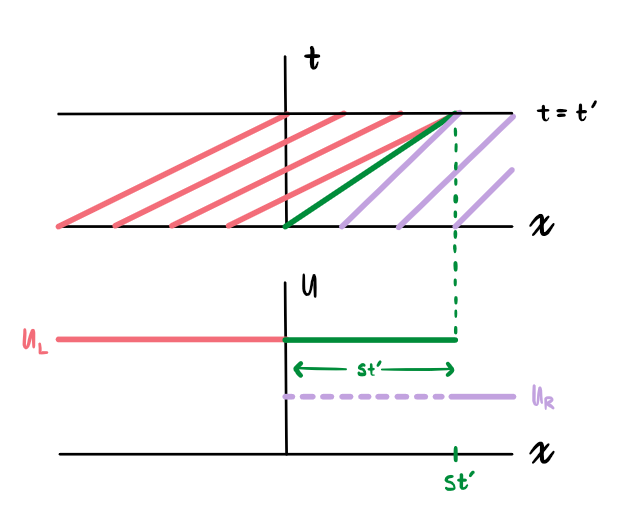
\includegraphics[width=1.0\textwidth]{riemann_shockwave.png}
        \caption{caption 1}
        \label{fig:shock}
    \end{subfigure}\hfill
    \begin{subfigure}{.48\textwidth}
        \centering
        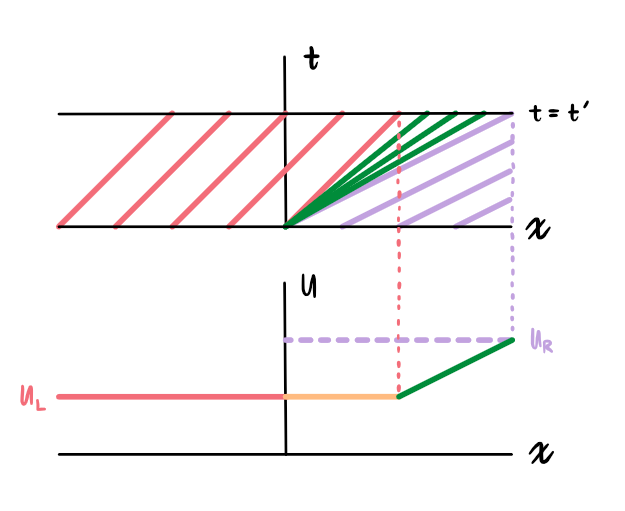
\includegraphics[width=1\textwidth]{riemann_rarefaction.png}
        \caption{caption 2}
        \label{fig:rarefaction}
    \end{subfigure}
    \caption{main caption}
    \label{fig:riemann_discontinuities}
\end{figure}

\subsection{Convergence}



\subsection{High-Resolution Methods}

shit i dont fully understand how to implement

\section{Experiments}

where our code crashed and burns

\subsection{`Easy' Problems}

basic riemann problems

\subsection{`Hard' Problems}

smooth curvy boies

\section{Conclusion}

this shit was way harder than i thought it would be

\newpage
\appendix
\section{Appendix}
\subsection{Code}

All project code can be found on our GitHub page: \url{https://github.com/agormann/MACM416-project}. As a courtesy, we have also included our code in this document, below.

[insert code]

\subsection{Analytical Solution via the Method of Characteristics}

We wish to solve the 1-D inviscid Burgers' equation analytically.

Given data on some curve $ \Gamma \subset \overline{\Omega} $, we are looking specific parametric curves $ (x(t), t) $ which connect points $(x, t) \in \Omega$ to $ \Gamma $. We want these curves to be precisely those which are parallel to the vector $(u, 1)$, that is
\[
    \frac{dx}{dt} = \frac{u(x(t), t)}{1} = u(x(t), t)
\]

Now supposing that $u$ solves (2), let $z(t)$ denote the value of $u$ along a characteristic, i.e. 
\[
    z(t) = u(x(t), t)
\]
Then by the chain rule
\[
    \frac{dz}{dt} = \partial_x u(x(t), t) \frac{dx}{dt}u(x(t), t) + \partial_t u(x(t), t)
\]
but $ x'(t) = u(x,t) $, so
\[
    \frac{dz}{dt} = \partial_t u(x(t), t) + u(x,t)\partial_x u(x(t), t)
\]
which is precisely 0 by (2). Hence, we have the following coupled system of ODEs
\begin{equation}
    \begin{cases}
        x'(t) = z(t) = u(x(t), t) \\
        z'(t) = 0
    \end{cases}
\end{equation}
Integrating the second term, we get that
\[
    z(t) = z_0
\]
for some $ z_0 \in \R $. But $z(t) = u(x(t), t)$, so then $u(x(t), t) = z_0$. This corroborates our findings with (3). Now by integrating the first term, we get
\begin{equation}
    x(t) = z_0t + x_0
\end{equation}
where $ x_0 \in \R $. Evaluating at $t=0$, we have that $x(0) = x_0$. Now assuming we are prescribed some initial condition $u(x,0) = g(x)$, we have that (5) becomes
\begin{equation}
    x(t) = g(x_0)t + x_0
\end{equation}
which are exactly those characteristic curves we initially sought.

% bibliography
\nocite{choksi2022}
\nocite{iserles2009}
% \nocite{kutz2013}
% \nocite{trefethen2001}
% \nocite{learncfd}
% \nocite{evans2010}
\nocite{leveque1992}
\nocite{leveque2002}
\printbibliography

\end{document}